
% Default to the notebook output style

    


% Inherit from the specified cell style.




    
\documentclass[11pt]{article}

    
    
    \usepackage[T1]{fontenc}
    % Nicer default font (+ math font) than Computer Modern for most use cases
    \usepackage{mathpazo}

    % Basic figure setup, for now with no caption control since it's done
    % automatically by Pandoc (which extracts ![](path) syntax from Markdown).
    \usepackage{graphicx}
    % We will generate all images so they have a width \maxwidth. This means
    % that they will get their normal width if they fit onto the page, but
    % are scaled down if they would overflow the margins.
    \makeatletter
    \def\maxwidth{\ifdim\Gin@nat@width>\linewidth\linewidth
    \else\Gin@nat@width\fi}
    \makeatother
    \let\Oldincludegraphics\includegraphics
    % Set max figure width to be 80% of text width, for now hardcoded.
    \renewcommand{\includegraphics}[1]{\Oldincludegraphics[width=.8\maxwidth]{#1}}
    % Ensure that by default, figures have no caption (until we provide a
    % proper Figure object with a Caption API and a way to capture that
    % in the conversion process - todo).
    \usepackage{caption}
    \DeclareCaptionLabelFormat{nolabel}{}
    \captionsetup{labelformat=nolabel}

    \usepackage{adjustbox} % Used to constrain images to a maximum size 
    \usepackage{xcolor} % Allow colors to be defined
    \usepackage{enumerate} % Needed for markdown enumerations to work
    \usepackage{geometry} % Used to adjust the document margins
    \usepackage{amsmath} % Equations
    \usepackage{amssymb} % Equations
    \usepackage{textcomp} % defines textquotesingle
    % Hack from http://tex.stackexchange.com/a/47451/13684:
    \AtBeginDocument{%
        \def\PYZsq{\textquotesingle}% Upright quotes in Pygmentized code
    }
    \usepackage{upquote} % Upright quotes for verbatim code
    \usepackage{eurosym} % defines \euro
    \usepackage[mathletters]{ucs} % Extended unicode (utf-8) support
    \usepackage[utf8x]{inputenc} % Allow utf-8 characters in the tex document
    \usepackage{fancyvrb} % verbatim replacement that allows latex
    \usepackage{grffile} % extends the file name processing of package graphics 
                         % to support a larger range 
    % The hyperref package gives us a pdf with properly built
    % internal navigation ('pdf bookmarks' for the table of contents,
    % internal cross-reference links, web links for URLs, etc.)
    \usepackage{hyperref}
    \usepackage{longtable} % longtable support required by pandoc >1.10
    \usepackage{booktabs}  % table support for pandoc > 1.12.2
    \usepackage[inline]{enumitem} % IRkernel/repr support (it uses the enumerate* environment)
    \usepackage[normalem]{ulem} % ulem is needed to support strikethroughs (\sout)
                                % normalem makes italics be italics, not underlines
    

    
    
    % Colors for the hyperref package
    \definecolor{urlcolor}{rgb}{0,.145,.698}
    \definecolor{linkcolor}{rgb}{.71,0.21,0.01}
    \definecolor{citecolor}{rgb}{.12,.54,.11}

    % ANSI colors
    \definecolor{ansi-black}{HTML}{3E424D}
    \definecolor{ansi-black-intense}{HTML}{282C36}
    \definecolor{ansi-red}{HTML}{E75C58}
    \definecolor{ansi-red-intense}{HTML}{B22B31}
    \definecolor{ansi-green}{HTML}{00A250}
    \definecolor{ansi-green-intense}{HTML}{007427}
    \definecolor{ansi-yellow}{HTML}{DDB62B}
    \definecolor{ansi-yellow-intense}{HTML}{B27D12}
    \definecolor{ansi-blue}{HTML}{208FFB}
    \definecolor{ansi-blue-intense}{HTML}{0065CA}
    \definecolor{ansi-magenta}{HTML}{D160C4}
    \definecolor{ansi-magenta-intense}{HTML}{A03196}
    \definecolor{ansi-cyan}{HTML}{60C6C8}
    \definecolor{ansi-cyan-intense}{HTML}{258F8F}
    \definecolor{ansi-white}{HTML}{C5C1B4}
    \definecolor{ansi-white-intense}{HTML}{A1A6B2}

    % commands and environments needed by pandoc snippets
    % extracted from the output of `pandoc -s`
    \providecommand{\tightlist}{%
      \setlength{\itemsep}{0pt}\setlength{\parskip}{0pt}}
    \DefineVerbatimEnvironment{Highlighting}{Verbatim}{commandchars=\\\{\}}
    % Add ',fontsize=\small' for more characters per line
    \newenvironment{Shaded}{}{}
    \newcommand{\KeywordTok}[1]{\textcolor[rgb]{0.00,0.44,0.13}{\textbf{{#1}}}}
    \newcommand{\DataTypeTok}[1]{\textcolor[rgb]{0.56,0.13,0.00}{{#1}}}
    \newcommand{\DecValTok}[1]{\textcolor[rgb]{0.25,0.63,0.44}{{#1}}}
    \newcommand{\BaseNTok}[1]{\textcolor[rgb]{0.25,0.63,0.44}{{#1}}}
    \newcommand{\FloatTok}[1]{\textcolor[rgb]{0.25,0.63,0.44}{{#1}}}
    \newcommand{\CharTok}[1]{\textcolor[rgb]{0.25,0.44,0.63}{{#1}}}
    \newcommand{\StringTok}[1]{\textcolor[rgb]{0.25,0.44,0.63}{{#1}}}
    \newcommand{\CommentTok}[1]{\textcolor[rgb]{0.38,0.63,0.69}{\textit{{#1}}}}
    \newcommand{\OtherTok}[1]{\textcolor[rgb]{0.00,0.44,0.13}{{#1}}}
    \newcommand{\AlertTok}[1]{\textcolor[rgb]{1.00,0.00,0.00}{\textbf{{#1}}}}
    \newcommand{\FunctionTok}[1]{\textcolor[rgb]{0.02,0.16,0.49}{{#1}}}
    \newcommand{\RegionMarkerTok}[1]{{#1}}
    \newcommand{\ErrorTok}[1]{\textcolor[rgb]{1.00,0.00,0.00}{\textbf{{#1}}}}
    \newcommand{\NormalTok}[1]{{#1}}
    
    % Additional commands for more recent versions of Pandoc
    \newcommand{\ConstantTok}[1]{\textcolor[rgb]{0.53,0.00,0.00}{{#1}}}
    \newcommand{\SpecialCharTok}[1]{\textcolor[rgb]{0.25,0.44,0.63}{{#1}}}
    \newcommand{\VerbatimStringTok}[1]{\textcolor[rgb]{0.25,0.44,0.63}{{#1}}}
    \newcommand{\SpecialStringTok}[1]{\textcolor[rgb]{0.73,0.40,0.53}{{#1}}}
    \newcommand{\ImportTok}[1]{{#1}}
    \newcommand{\DocumentationTok}[1]{\textcolor[rgb]{0.73,0.13,0.13}{\textit{{#1}}}}
    \newcommand{\AnnotationTok}[1]{\textcolor[rgb]{0.38,0.63,0.69}{\textbf{\textit{{#1}}}}}
    \newcommand{\CommentVarTok}[1]{\textcolor[rgb]{0.38,0.63,0.69}{\textbf{\textit{{#1}}}}}
    \newcommand{\VariableTok}[1]{\textcolor[rgb]{0.10,0.09,0.49}{{#1}}}
    \newcommand{\ControlFlowTok}[1]{\textcolor[rgb]{0.00,0.44,0.13}{\textbf{{#1}}}}
    \newcommand{\OperatorTok}[1]{\textcolor[rgb]{0.40,0.40,0.40}{{#1}}}
    \newcommand{\BuiltInTok}[1]{{#1}}
    \newcommand{\ExtensionTok}[1]{{#1}}
    \newcommand{\PreprocessorTok}[1]{\textcolor[rgb]{0.74,0.48,0.00}{{#1}}}
    \newcommand{\AttributeTok}[1]{\textcolor[rgb]{0.49,0.56,0.16}{{#1}}}
    \newcommand{\InformationTok}[1]{\textcolor[rgb]{0.38,0.63,0.69}{\textbf{\textit{{#1}}}}}
    \newcommand{\WarningTok}[1]{\textcolor[rgb]{0.38,0.63,0.69}{\textbf{\textit{{#1}}}}}
    
    
    % Define a nice break command that doesn't care if a line doesn't already
    % exist.
    \def\br{\hspace*{\fill} \\* }
    % Math Jax compatability definitions
    \def\gt{>}
    \def\lt{<}
    % Document parameters
    \title{Opening the black box of Deep Neural Networks with More Information}
    
    
    

    % Pygments definitions
    
\makeatletter
\def\PY@reset{\let\PY@it=\relax \let\PY@bf=\relax%
    \let\PY@ul=\relax \let\PY@tc=\relax%
    \let\PY@bc=\relax \let\PY@ff=\relax}
\def\PY@tok#1{\csname PY@tok@#1\endcsname}
\def\PY@toks#1+{\ifx\relax#1\empty\else%
    \PY@tok{#1}\expandafter\PY@toks\fi}
\def\PY@do#1{\PY@bc{\PY@tc{\PY@ul{%
    \PY@it{\PY@bf{\PY@ff{#1}}}}}}}
\def\PY#1#2{\PY@reset\PY@toks#1+\relax+\PY@do{#2}}

\expandafter\def\csname PY@tok@w\endcsname{\def\PY@tc##1{\textcolor[rgb]{0.73,0.73,0.73}{##1}}}
\expandafter\def\csname PY@tok@c\endcsname{\let\PY@it=\textit\def\PY@tc##1{\textcolor[rgb]{0.25,0.50,0.50}{##1}}}
\expandafter\def\csname PY@tok@cp\endcsname{\def\PY@tc##1{\textcolor[rgb]{0.74,0.48,0.00}{##1}}}
\expandafter\def\csname PY@tok@k\endcsname{\let\PY@bf=\textbf\def\PY@tc##1{\textcolor[rgb]{0.00,0.50,0.00}{##1}}}
\expandafter\def\csname PY@tok@kp\endcsname{\def\PY@tc##1{\textcolor[rgb]{0.00,0.50,0.00}{##1}}}
\expandafter\def\csname PY@tok@kt\endcsname{\def\PY@tc##1{\textcolor[rgb]{0.69,0.00,0.25}{##1}}}
\expandafter\def\csname PY@tok@o\endcsname{\def\PY@tc##1{\textcolor[rgb]{0.40,0.40,0.40}{##1}}}
\expandafter\def\csname PY@tok@ow\endcsname{\let\PY@bf=\textbf\def\PY@tc##1{\textcolor[rgb]{0.67,0.13,1.00}{##1}}}
\expandafter\def\csname PY@tok@nb\endcsname{\def\PY@tc##1{\textcolor[rgb]{0.00,0.50,0.00}{##1}}}
\expandafter\def\csname PY@tok@nf\endcsname{\def\PY@tc##1{\textcolor[rgb]{0.00,0.00,1.00}{##1}}}
\expandafter\def\csname PY@tok@nc\endcsname{\let\PY@bf=\textbf\def\PY@tc##1{\textcolor[rgb]{0.00,0.00,1.00}{##1}}}
\expandafter\def\csname PY@tok@nn\endcsname{\let\PY@bf=\textbf\def\PY@tc##1{\textcolor[rgb]{0.00,0.00,1.00}{##1}}}
\expandafter\def\csname PY@tok@ne\endcsname{\let\PY@bf=\textbf\def\PY@tc##1{\textcolor[rgb]{0.82,0.25,0.23}{##1}}}
\expandafter\def\csname PY@tok@nv\endcsname{\def\PY@tc##1{\textcolor[rgb]{0.10,0.09,0.49}{##1}}}
\expandafter\def\csname PY@tok@no\endcsname{\def\PY@tc##1{\textcolor[rgb]{0.53,0.00,0.00}{##1}}}
\expandafter\def\csname PY@tok@nl\endcsname{\def\PY@tc##1{\textcolor[rgb]{0.63,0.63,0.00}{##1}}}
\expandafter\def\csname PY@tok@ni\endcsname{\let\PY@bf=\textbf\def\PY@tc##1{\textcolor[rgb]{0.60,0.60,0.60}{##1}}}
\expandafter\def\csname PY@tok@na\endcsname{\def\PY@tc##1{\textcolor[rgb]{0.49,0.56,0.16}{##1}}}
\expandafter\def\csname PY@tok@nt\endcsname{\let\PY@bf=\textbf\def\PY@tc##1{\textcolor[rgb]{0.00,0.50,0.00}{##1}}}
\expandafter\def\csname PY@tok@nd\endcsname{\def\PY@tc##1{\textcolor[rgb]{0.67,0.13,1.00}{##1}}}
\expandafter\def\csname PY@tok@s\endcsname{\def\PY@tc##1{\textcolor[rgb]{0.73,0.13,0.13}{##1}}}
\expandafter\def\csname PY@tok@sd\endcsname{\let\PY@it=\textit\def\PY@tc##1{\textcolor[rgb]{0.73,0.13,0.13}{##1}}}
\expandafter\def\csname PY@tok@si\endcsname{\let\PY@bf=\textbf\def\PY@tc##1{\textcolor[rgb]{0.73,0.40,0.53}{##1}}}
\expandafter\def\csname PY@tok@se\endcsname{\let\PY@bf=\textbf\def\PY@tc##1{\textcolor[rgb]{0.73,0.40,0.13}{##1}}}
\expandafter\def\csname PY@tok@sr\endcsname{\def\PY@tc##1{\textcolor[rgb]{0.73,0.40,0.53}{##1}}}
\expandafter\def\csname PY@tok@ss\endcsname{\def\PY@tc##1{\textcolor[rgb]{0.10,0.09,0.49}{##1}}}
\expandafter\def\csname PY@tok@sx\endcsname{\def\PY@tc##1{\textcolor[rgb]{0.00,0.50,0.00}{##1}}}
\expandafter\def\csname PY@tok@m\endcsname{\def\PY@tc##1{\textcolor[rgb]{0.40,0.40,0.40}{##1}}}
\expandafter\def\csname PY@tok@gh\endcsname{\let\PY@bf=\textbf\def\PY@tc##1{\textcolor[rgb]{0.00,0.00,0.50}{##1}}}
\expandafter\def\csname PY@tok@gu\endcsname{\let\PY@bf=\textbf\def\PY@tc##1{\textcolor[rgb]{0.50,0.00,0.50}{##1}}}
\expandafter\def\csname PY@tok@gd\endcsname{\def\PY@tc##1{\textcolor[rgb]{0.63,0.00,0.00}{##1}}}
\expandafter\def\csname PY@tok@gi\endcsname{\def\PY@tc##1{\textcolor[rgb]{0.00,0.63,0.00}{##1}}}
\expandafter\def\csname PY@tok@gr\endcsname{\def\PY@tc##1{\textcolor[rgb]{1.00,0.00,0.00}{##1}}}
\expandafter\def\csname PY@tok@ge\endcsname{\let\PY@it=\textit}
\expandafter\def\csname PY@tok@gs\endcsname{\let\PY@bf=\textbf}
\expandafter\def\csname PY@tok@gp\endcsname{\let\PY@bf=\textbf\def\PY@tc##1{\textcolor[rgb]{0.00,0.00,0.50}{##1}}}
\expandafter\def\csname PY@tok@go\endcsname{\def\PY@tc##1{\textcolor[rgb]{0.53,0.53,0.53}{##1}}}
\expandafter\def\csname PY@tok@gt\endcsname{\def\PY@tc##1{\textcolor[rgb]{0.00,0.27,0.87}{##1}}}
\expandafter\def\csname PY@tok@err\endcsname{\def\PY@bc##1{\setlength{\fboxsep}{0pt}\fcolorbox[rgb]{1.00,0.00,0.00}{1,1,1}{\strut ##1}}}
\expandafter\def\csname PY@tok@kc\endcsname{\let\PY@bf=\textbf\def\PY@tc##1{\textcolor[rgb]{0.00,0.50,0.00}{##1}}}
\expandafter\def\csname PY@tok@kd\endcsname{\let\PY@bf=\textbf\def\PY@tc##1{\textcolor[rgb]{0.00,0.50,0.00}{##1}}}
\expandafter\def\csname PY@tok@kn\endcsname{\let\PY@bf=\textbf\def\PY@tc##1{\textcolor[rgb]{0.00,0.50,0.00}{##1}}}
\expandafter\def\csname PY@tok@kr\endcsname{\let\PY@bf=\textbf\def\PY@tc##1{\textcolor[rgb]{0.00,0.50,0.00}{##1}}}
\expandafter\def\csname PY@tok@bp\endcsname{\def\PY@tc##1{\textcolor[rgb]{0.00,0.50,0.00}{##1}}}
\expandafter\def\csname PY@tok@fm\endcsname{\def\PY@tc##1{\textcolor[rgb]{0.00,0.00,1.00}{##1}}}
\expandafter\def\csname PY@tok@vc\endcsname{\def\PY@tc##1{\textcolor[rgb]{0.10,0.09,0.49}{##1}}}
\expandafter\def\csname PY@tok@vg\endcsname{\def\PY@tc##1{\textcolor[rgb]{0.10,0.09,0.49}{##1}}}
\expandafter\def\csname PY@tok@vi\endcsname{\def\PY@tc##1{\textcolor[rgb]{0.10,0.09,0.49}{##1}}}
\expandafter\def\csname PY@tok@vm\endcsname{\def\PY@tc##1{\textcolor[rgb]{0.10,0.09,0.49}{##1}}}
\expandafter\def\csname PY@tok@sa\endcsname{\def\PY@tc##1{\textcolor[rgb]{0.73,0.13,0.13}{##1}}}
\expandafter\def\csname PY@tok@sb\endcsname{\def\PY@tc##1{\textcolor[rgb]{0.73,0.13,0.13}{##1}}}
\expandafter\def\csname PY@tok@sc\endcsname{\def\PY@tc##1{\textcolor[rgb]{0.73,0.13,0.13}{##1}}}
\expandafter\def\csname PY@tok@dl\endcsname{\def\PY@tc##1{\textcolor[rgb]{0.73,0.13,0.13}{##1}}}
\expandafter\def\csname PY@tok@s2\endcsname{\def\PY@tc##1{\textcolor[rgb]{0.73,0.13,0.13}{##1}}}
\expandafter\def\csname PY@tok@sh\endcsname{\def\PY@tc##1{\textcolor[rgb]{0.73,0.13,0.13}{##1}}}
\expandafter\def\csname PY@tok@s1\endcsname{\def\PY@tc##1{\textcolor[rgb]{0.73,0.13,0.13}{##1}}}
\expandafter\def\csname PY@tok@mb\endcsname{\def\PY@tc##1{\textcolor[rgb]{0.40,0.40,0.40}{##1}}}
\expandafter\def\csname PY@tok@mf\endcsname{\def\PY@tc##1{\textcolor[rgb]{0.40,0.40,0.40}{##1}}}
\expandafter\def\csname PY@tok@mh\endcsname{\def\PY@tc##1{\textcolor[rgb]{0.40,0.40,0.40}{##1}}}
\expandafter\def\csname PY@tok@mi\endcsname{\def\PY@tc##1{\textcolor[rgb]{0.40,0.40,0.40}{##1}}}
\expandafter\def\csname PY@tok@il\endcsname{\def\PY@tc##1{\textcolor[rgb]{0.40,0.40,0.40}{##1}}}
\expandafter\def\csname PY@tok@mo\endcsname{\def\PY@tc##1{\textcolor[rgb]{0.40,0.40,0.40}{##1}}}
\expandafter\def\csname PY@tok@ch\endcsname{\let\PY@it=\textit\def\PY@tc##1{\textcolor[rgb]{0.25,0.50,0.50}{##1}}}
\expandafter\def\csname PY@tok@cm\endcsname{\let\PY@it=\textit\def\PY@tc##1{\textcolor[rgb]{0.25,0.50,0.50}{##1}}}
\expandafter\def\csname PY@tok@cpf\endcsname{\let\PY@it=\textit\def\PY@tc##1{\textcolor[rgb]{0.25,0.50,0.50}{##1}}}
\expandafter\def\csname PY@tok@c1\endcsname{\let\PY@it=\textit\def\PY@tc##1{\textcolor[rgb]{0.25,0.50,0.50}{##1}}}
\expandafter\def\csname PY@tok@cs\endcsname{\let\PY@it=\textit\def\PY@tc##1{\textcolor[rgb]{0.25,0.50,0.50}{##1}}}

\def\PYZbs{\char`\\}
\def\PYZus{\char`\_}
\def\PYZob{\char`\{}
\def\PYZcb{\char`\}}
\def\PYZca{\char`\^}
\def\PYZam{\char`\&}
\def\PYZlt{\char`\<}
\def\PYZgt{\char`\>}
\def\PYZsh{\char`\#}
\def\PYZpc{\char`\%}
\def\PYZdl{\char`\$}
\def\PYZhy{\char`\-}
\def\PYZsq{\char`\'}
\def\PYZdq{\char`\"}
\def\PYZti{\char`\~}
% for compatibility with earlier versions
\def\PYZat{@}
\def\PYZlb{[}
\def\PYZrb{]}
\makeatother


    % Exact colors from NB
    \definecolor{incolor}{rgb}{0.0, 0.0, 0.5}
    \definecolor{outcolor}{rgb}{0.545, 0.0, 0.0}



    
    % Prevent overflowing lines due to hard-to-break entities
    \sloppy 
    % Setup hyperref package
    \hypersetup{
      breaklinks=true,  % so long urls are correctly broken across lines
      colorlinks=true,
      urlcolor=urlcolor,
      linkcolor=linkcolor,
      citecolor=citecolor,
      }
    % Slightly bigger margins than the latex defaults
    
    \geometry{verbose,tmargin=1in,bmargin=1in,lmargin=1in,rmargin=1in}
    
    

    \begin{document}

    \maketitle
    
    \begin{abstract}

    A lot of methods and approaches exist for effective training and application of neural networks, however they are still not well understood theoretically. In this project we explore the evolution of various neural networks trained with stochastic gradient descent using information plane approach proposed by Schwartz-Ziv and Tishby, replicate their experiments as well as introduce our own modifications.

    \end{abstract}

    
    \section{Introduction and related
work}\label{introduction-and-related-work}

    Although neural networks have proven to be invaluable in research as
well as in automating various business processes, a lot of questions
remain open as to how they work and why they are so effective. One model
developed (by \emph{Shwartz Ziv, Tishby}) to answer them is the
\textbf{information plane}

    From a statistical point of view, the data \(X\) and labels \(Y\) used
to train a neural network that outputs prediction \(\hat Y\) are two
random variables drawn from some unknown distribution. The
\emph{activation value} (output of the activation function) of each
layer of the network \(T_i \in \{T_1,T_2,...,T_n=\hat Y\}\) is a
function of \(X\) and, thus, a random variable as well.

    As a way to understand this sequence of random variables, the original
paper by \emph{Schwartz-Ziv and Tishby} proposes using \emph{mutual
information}:

\[
MI(X;Y) = - \sum_{x,y} p(x,y) \log \frac{p(x,y)}{p(x)p(y)}
\]

where \(X\),\(Y\) are distributions and \(p(x)\), \(p(y)\), \(p(x,y)\)
are probability mass functions

Every layer \(T_i\) of a neural network thus is a point in the
\textbf{information plane}: \((MI(X;T_i),MI(T_i;Y))\) where
\(MI(X;T_i) \geq MI(X; T_{i+1})\) and \(MI(T_i; Y) \geq MI(T_{i+1};Y)\).
This gives rise to an intuitive model of neural network being an
\textbf{information funnel} that layer by layer extracts the most
\emph{relevant} (informative of \(Y\)) information out of \(X\) and
discards the rest.

    \emph{Schwartz-Ziv and Tishby} present certain that support the
information funnel model as well as demonstrate that the process of
\emph{Stochastic Gradient Descent} for a neural network tends to
decompose into 2 stages: 
\begin{itemize}
\item Fitting the network to the data ("moving the
funnel"). During this stage \(MI(\hat Y; Y)\) and \(MI(\hat Y; X)\)
grow. 
\item Compressing the output of the network ("shrinking the funnel").
During this stage \(MI(\hat Y; Y)\) grows slower and \(MI(\hat Y; X)\)
shrinks.
\end{itemize}

    \textbf{Our goal} in this project is to replicate these experiments as
well as further explore this model with our own tools and experiments

    \section{Experiments}\label{experiments}

    Please note, that we ran a lot more than 3 experiments in the process of
preparing this report, but here we omit small modifications of
experimental setup that don't change the output as they are remarkably
not interesting to read. Because of the 5-page limit, the jupyter notebook has more experiments, than the text report

    \subsection{Estimating mutual
information}\label{estimating-mutual-information}

    According to the formula

\[
MI(X;Y) = - \sum_{x,y} p(x,y) \log \frac{p(x,y)}{p(x)p(y)}
\]

in order to estimate the mutual information between \(X\), \(Y\) and a
layer, one \emph{simply} needs to estimate \(p(x)\), \(p(y)\) and
\(p(x,y)\) for all \(x\) and \(y\). Thus, we need The following
procedure is used (\textbf{but not described}, one has to look through
the code attached to the paper to find that out) in the original paper:
1. Given dataset X, Y estimate
\(p(x)=\frac{\text{count}(X=x)}{\text{count}(X)}\),
\(p(y)=\frac{\text{count}(Y=y)}{\text{count}(Y)}\) as well as joint
\(p(x,y)=\frac{\text{count}(X=x,Y=y)}{\text{count}(X,Y)}\) 2. Run
\emph{all} data points \(x\) in \(X\) through the neural network, obtain
\(T_i\) for all \(i\) 3. Repeat step 1 for every (\(T_i\), \(X\))

    Note that this approach requires all random variales to be discrete,
hence the activation values of neurons have to be discretized

    Because the procedure is not described in the paper and the code is very
hard to parse, we had to give up the idea of re-implementing it and make
heavy use of it's API. However, we did implement an improvement upon the
original estimation approach:

    \subsubsection{Extended MI estimator}\label{extended-mi-estimator}

    The model described above treats \(X\), \(Y\) and \(T_i\) as random
variables, but assumes the function \(T(X)\) is completely
deterministic. Which it is not, because we are training the neural
network with \emph{stochastic gradient descent}: every time we retrain
it, the results will be slightly different.

We have implemented an MI estimator that accounts for this. Instead of
working with one neural network, we can train several and sample
elements of \(T_i\) (activation values of neurons) randomly from several
\(T_{ij}\) (\(i\) - layer, \(j\) - index). From now on, this will be
called \emph{extended MI estimator} and the original approach with one
network - \emph{simple MI estimator}. We will demonstrate the benefits
of this approach further.

    \subsection{Experimental setup}\label{experimental-setup}

Every experiment was conducted as follows: 
\begin{itemize}
\item Several copies of a neural
network with identical architecture (number, size and type of layers)
are created. 
\item They are trained iteratively using pytorch implementation
of \emph{Stochastic Gradient Descent} 
\irem After each iteration of the
algorithm, the full procedure \emph{extended MI estimator} is run and
the estimated mutual information \(MI(X;T_i)\), \(MI(T_i;Y)\) is plotted
on a graphical representation fo the \textbf{information plane}
\end{itemize}

Note that MI estimation is much more resource intensive than SGD itself
and it doesn't run on the GPU. For this reason, going from primitive
multi-layer perceptrons to experiments with more complicated neural
networks is \emph{very hard}.

    \subsection{Data}\label{data}

    In order to replicate \emph{Tishby an Schwartz-Ziv's} original
experiment, we'll generate synthetic test data using 
\begin{itemize}
\item a simple binary
decision function with small Gaussian noise. 
\item another, more complicated decision function, in order to compare the
results.
\item and finally, MNIST dataset of hand-written digits, to test if the
results generalize from the synthetic dataset to a more realistic one
\end{itemize}

    \subsection{Experiment 2: As close to Tishby setup as
possible}\label{experiment-2-as-close-to-tishby-setup-as-possible}

    Six-layer perceptron, simple MI estimator, simple synthetic dataset

    \begin{center}
    \adjustimage{max size={0.9\linewidth}{0.9\paperheight}}{output_37_1.png}
    \end{center}
    { \hspace*{\fill} \\}

    Different colors represent different layers of the neural network. As
one can see, this network is too simple for the observations of
\emph{Schvartz-Ziv and Tishby} to manifest.
    
    For comparison, here are the results from the original paper:

\begin{figure}
\centering
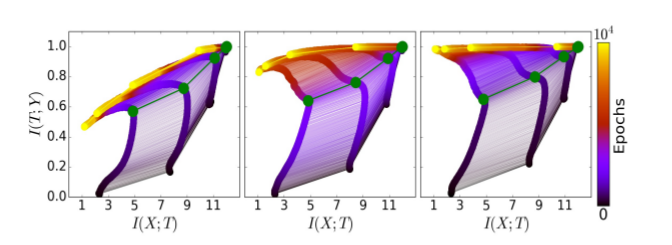
\includegraphics{2stages.png}
\caption{2 Stages}
\end{figure}

    Indeed, the experiment reproduces successfully. But what if we use the
same network architecture and the same data, but with our \emph{extended
MI estimator} ?

    \begin{center}
    \adjustimage{max size={0.9\linewidth}{0.9\paperheight}}{output_40_1.png}
    \end{center}
    { \hspace*{\fill} \\}
    
    Feel free to take a second to process the awe and admiration of this
clearly superior method you are experiencing at the moment.

    \subsection{Experiment 4: (Almost) Real-world
problem}\label{experiment-4-almost-real-world-problem}

    For this experiment we will use: 
\begin{enumerate} 
\item MNIST dataset of hand-written digits
\item Convolutional neural network (1 conv layer, 1 ReLU layer, 2 fully
connected layer) roughly inspired by \emph{Cireşan} et al 
\item Extended mutual information estimator
\end{enumerate}
            
    \begin{center}
    \adjustimage{max size={0.9\linewidth}{0.9\paperheight}}{output_49_3.png}
    \end{center}
    { \hspace*{\fill} \\}
    
    \subsection{Bonus: mutual information stopping
criterion}\label{bonus-mutual-information-stopping-criterion}

    It felt wrong to end this project without a more or less practical (i.e.
code you can use) result, so here it is: an algorithm for training
neural networks that uses mutual information profile of the last layer
\(I(X; \hat Y) - \beta I(\hat Y; Y)\) as its stopping criterion.
Because, as already mentioned, MI estimators are very slow, we do not
check this criterion at every iteration.

Code is attached

    \subsection{Conclusions}\label{conclusions}

    \begin{itemize}
\tightlist
\item
  Original experiment \textbf{replicated successfuly}
\item
  Small changes to the original experiment didn't change the results,
  but on very different (like the convolutional one) neural networks,
  the experiment turned out hard to reproduce. However, we cannot
  conclude that \emph{Shwartz-Ziv and Tishby's} results were erroneous ,
  because there are other possible explanations like not having enough
  time and resources to run the experiment till stage 2
\end{itemize}

We have also introduced: 
\begin{itemize}
\item An improvement of the mutual information
estimator with several neural networks 
\item A new stopping criterion for
neural network optimization
\end{itemize}

    \section{Contributions}\label{contributions}

    \begin{itemize}
\tightlist
\item
  \textbf{Vadim} - almost everything
\item
  \textbf{Leonid} - a few slides, thoughts and prayers, valuable
  feedback
\end{itemize}

    \section{References}\label{references}

    \begin{itemize}
\tightlist
\item
  \emph{Ravid Shwartz-Ziv, Naftali Tishby} Opening the Black Box of Deep
  Neural Networks via Information
\item
  \emph{Dan C. Cireşan, Ueli Meier, Jonathan Masci, Luca M. Gambardella,
  Jürgen Schmidhuber} Flexible, High Performance Convolutional Neural
  Networks for Image Classification
\end{itemize}


    % Add a bibliography block to the postdoc
    
    
    
    \end{document}
